% !TEX root = knottedMain.tex
\documentclass[varwidth=\maxdimen]{standalone}

\usepackage{mathtools,amssymb,mathrsfs,dutchcal,upgreek,faktor,accents,etoolbox,multicol}
\usepackage[dvipsnames]{xcolor}
\definecolor{mygreen}{RGB}{	8,156,79 }
\usepackage{tikz,tikz-cd}
\usetikzlibrary{patterns,knots,arrows.meta,decorations.markings}
\tikzset{>={Straight Barb[scale=0.85]}}
\tikzcdset{
  cells={font=\everymath\expandafter{\the\everymath\displaystyle}},
  arrow style=tikz,
  diagrams={>={Straight Barb[scale=0.85]}},
  every label/.append style = {font = \small}
}


\begin{document}
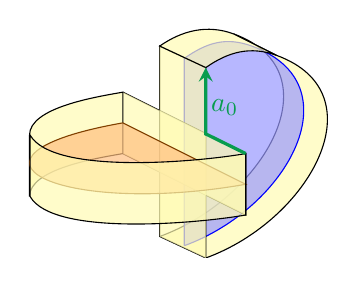
\begin{tikzpicture}[scale=0.78,fill opacity=0.7]
       \clip (-1.55,-1.2) rectangle (3.35,2.55);
        %vertical band vertical piece
        \fill[yellow!30!,draw=black]
            (1.35,-1.2)  to[out=20,in=-20,distance=1.8cm] (2.5,2.1)
            -- (1.8,2.45) to[out=-20,in=20,distance=1.8cm]  (0.6,-0.85) ;
        %middle vertical disk
        \fill[blue!40!,draw=blue]
            (1,-1) -- (1,2.05) to[out=35,in=160,distance=0.45cm] (2.1,2.25)
            to[out=-20,in=20,distance=1.8cm]  (1,-1) ;
        %vertical flat
        \draw[black] (0.6,-0.85) -- (1.35,-1.2) -- (1.35,1.9) -- (0.6,2.25) --  cycle ;
        %horizontal flat
        \draw[black] (0,1.5) -- (2,0.5) -- (2,-0.5) -- (0,0.5) ;
        %vertical flat
        \fill[yellow!30!,opacity=0.7](0.6,-0.85) -- (1.35,-1.2) -- (1.35,1.9) -- (0.6,2.25) --  cycle ;
        %horizontal flat
        \fill[yellow!30!,opacity=0.7] (0,1.5) -- (2,0.5) -- (2,-0.5) -- (0,0.5) ;
        %back band
        \fill[yellow!30!,draw=black]
        (0,0.5) to[out=-170, in=90, distance=0.45cm] (-1.52,-0.2)
        -- (-1.52,0.8) to[out=90, in=-170, distance=0.45cm] (0,1.5) -- (0,0.5) ;
        %vertical band horizontal piece
        \fill[yellow!30!,draw=black]
            (1.35,1.9) -- (0.6,2.25) to[out=35,in=160,distance=0.45cm] (1.8,2.45)
            -- (2.5,2.1) to[out=160,in=35,distance=0.45cm] (1.35,1.9) ;
        % middle horizontal disk
        \fill[orange!50!,draw=orange!50!black]
            (0,1) to[out=-170,in=-170,distance=3.1cm] (2,0) -- (0,1) ;
        %horizontal band
        \fill[yellow!30!,draw=black]
            (-1.51,-0.2) to[out=-60,in=-170,distance=0.76cm] (2,-0.5)
            -- (2,0.5) to[out=-170,in=-60,distance=0.76cm] (-1.51,0.8) --(-1.51,-0.2) ;
        \draw[-stealth,mygreen,very thick,opacity=1] (2,0.5) -- (1.35,0.82) -- (1.35, 1.9) node[pos=0.4,right=-2pt]{$a_0$};
\end{tikzpicture}
    \qquad
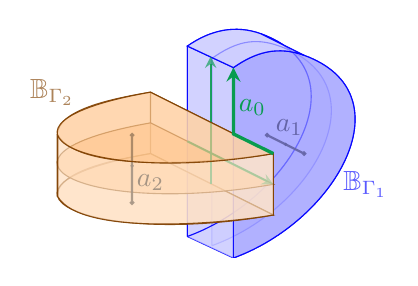
\begin{tikzpicture}[scale=0.78,fill opacity=0.65,draw opacity=0.9]
       \clip (-2,-1.2) rectangle (3.9,2.55);
       \draw[orange!50!black] 
            (-1.6,1.5) node[]{$\mathbb{B}_{\Gamma_2}$};
        \draw[blue]
            (3.5,0) node[]{$\mathbb{B}_{\Gamma_1}$};
        %back disk
        \fill[blue!20!,draw=blue]
            (0.6,-0.85) -- (0.6,2.25) to[out=35,in=160,distance=0.45cm] (1.8,2.45)
            to[out=-20,in=20,distance=1.8cm]  (0.6,-0.85) ;
        % middle vertical disk
        \fill[blue!20!,draw=blue]
            (1,-1) -- (1,2.05) to[out=35,in=160,distance=0.45cm] (2.1,2.25)
            to[out=-20,in=20,distance=1.8cm]  (1,-1) ;
        %vertical flat
        \fill[blue!20!,draw=blue]
            (0.6,-0.85) -- (1.35,-1.2) -- (1.35,1.9) -- (0.6,2.25) --  cycle ;
        %vertical band vertical piece
        \fill[blue!20!,draw=blue]
            (1.35,-1.2)  to[out=20,in=-20,distance=1.8cm] (2.5,2.1)
            -- (1.8,2.45) to[out=-20,in=20,distance=1.8cm]  (0.6,-0.85) ;
        % a_1
        \fill[draw,thick]
            (2.5,0.5) circle (0.5pt) -- 
            (1.9,0.8)  circle (0.5pt) node[pos=0.4,above,opacity=1]{$a_1$};
        \draw (2.2,0.65)  circle (0.5pt);
        %front disk
        \fill[blue!40!,draw=blue]
            (1.35,-1.2) -- (1.35,1.9) to[out=35,in=160,distance=0.45cm] (2.5,2.1)
            to[out=-20,in=20,distance=1.8cm] (1.35,-1.2) ;
        %horizontal flat
        \fill[orange!20!,draw=orange!50!black]
            (0,1.5) -- (2,0.5) -- (2,-0.5) -- (0,0.5) ;
        %back band
        \fill[orange!20!,draw=orange!50!black]
            (0,0.5) to[out=-170, in=90, distance=0.45cm] (-1.52,-0.2)
            -- (-1.52,0.8) to[out=90, in=-170, distance=0.45cm] (0,1.5) -- (0,0.5) ;
        %lower disk
        \fill[orange!30!,draw=orange!50!black]
            (0,0.5) to[out=-170,in=-170,distance=3.1cm] (2,-0.5)
            -- (0,0.5) ;
        % middle horizontal disk
        \fill[orange!50!,draw=orange!50!black]
            (0,1) to[out=-170,in=-170,distance=3.1cm] (2,0) -- (0,1) ;
        %vertical band horizontal piece
        \fill[blue!20!,draw=blue]
            (1.35,1.9) -- (0.6,2.25) to[out=35,in=160,distance=0.45cm] (1.8,2.45)
            -- (2.5,2.1) to[out=160,in=35,distance=0.45cm] (1.35,1.9) ;
        % green arcs
        \draw[-stealth,mygreen,thick]  
            (0.6,0.7) -- (2,0);
        \draw[-stealth,mygreen,thick] 
            (0.98,0) -- (0.98,2.08);
        % a_2
        \fill[draw,thick]
            (-0.3,-0.3) circle (0.5pt) -- 
            (-0.3,0.8)  circle (0.5pt) node[pos=0.3,right=-2pt,opacity=1]{$a_2$};
        \draw (-0.3,0.3)  circle (0.5pt);
        % orange lying band
        \fill[orange!20!,draw=orange!50!black]
            (-1.51,-0.2) to[out=-60,in=-170,distance=0.76cm] (2,-0.5)
            -- (2,0.5) to[out=-170,in=-60,distance=0.76cm] (-1.51,0.8) --(-1.51,-0.2)  ;
        %upper disk
        \fill[orange!40!,draw=orange!50!black]
            (2,0.5) to[out=-170,in=-170,distance=3.1cm] (0,1.5) -- (2,0.5) ;
        \draw[-stealth,mygreen,very thick,opacity=1] 
            (2,0.5) -- (1.35,0.82) -- (1.35, 1.9) node[pos=0.4,right=-2pt]{$a_0$} ;
\end{tikzpicture}
\end{document}